\documentclass[aspectratio=1610,t]{beamer}

\usepackage[english]{babel}
\usepackage{hyperref}
\usepackage{minted}
\usepackage{alltt}
\usepackage{amsmath}
\usepackage{graphicx}
\usepackage{xcolor}
\usepackage[utf-8]{inputenc}

\usetheme{metropolis}
\usemintedstyle{xcode}
\definecolor{codebg}{RGB}{247, 247, 246}
\setbeamercolor{background canvas}{bg=white}
\hypersetup{colorlinks,linkcolor=,urlcolor=orange}

\title{Lecture 3: Traits. Interior mutability}
\date{March 8, 2022}
\author{Alexander Stanovoy}
\institute{alex.stanovoy@gmail.com}

\begin{document}

% ----------------------------------------------------------------- %

\begin{frame}
\maketitle
\end{frame}

% ----------------------------------------------------------------- %

\begin{frame}[fragile]
\frametitle{In this lecture}
\begin{itemize}
    \item Traits
    \item Exotically Sized Types
    \item Standard library traits
    \item Comparision of traits with C++ capabilities
    \item Interior mutability: \texttt{Cell} and \texttt{RefCell}
\end{itemize}
\end{frame}

% ----------------------------------------------------------------- %

\begin{frame}[c]
\centering\Huge\textbf{Traits}
\end{frame}

% ----------------------------------------------------------------- %

\begin{frame}[fragile]
\frametitle{Traits}
In Rust, a trait is \textit{similar to} an interface in other languages. It's the way how we can define \textit{shared behavior} (i.e similarities between objects).

\begin{minted}[fontsize=\small]{rust}
    pub trait Animal {
        // No 'pub' keyword
        fn name(&self) -> String;
        fn noise(&self) -> String;

        // Traits can provide default method definitions
        fn talk(&self) {
            println!("{} says {}", self.name(), self.noise());
        }
    }
\end{minted}

Let's define some structures and implement this trait for them.
\end{frame}

% ----------------------------------------------------------------- %

\begin{frame}[fragile]
\frametitle{Traits}
\begin{minted}{rust}
    pub struct Sheep {
        name: String,
    }

    impl Animal for Sheep {
        // No 'pub' keyword
        fn name(&self) -> String {
            self.name.clone()
        }

        fn noise(&self) -> String {
            "baaaaah!".to_string()
        }
    }
\end{minted}
\end{frame}

% ----------------------------------------------------------------- %

\begin{frame}[fragile]
\frametitle{Traits}
Usage example:

\begin{minted}{rust}
    let sheep = Sheep {
        name: "Dolly".to_string(),
    };
    assert_eq!(sheep.name(), "Dolly");
    sheep.talk();  // prints 'Dolly says baaaaah!'
\end{minted}
\end{frame}

% ----------------------------------------------------------------- %

\begin{frame}[fragile]
\frametitle{Traits}
\begin{minted}[fontsize=\small]{rust}
    pub struct Dog {
        name: String,
    }

    impl Animal for Dog {
        fn name(&self) -> String { self.name.clone() }

        fn noise(&self) -> String {
            "ruff!".to_string()
        }

        // Default trait methods can be overridden.
        fn talk(&self) {
            println!("Ruff! Don't call me doggo");
        }
    }
\end{minted}
\end{frame}

% ----------------------------------------------------------------- %

\begin{frame}[fragile]
\frametitle{Traits: \texttt{where} keyword}
This will compile just fine:

\begin{minted}[fontsize=\small]{rust}
    #[derive(Clone)]
    pub struct Human { name: String }

    impl Animal for Human {
        fn name(&self) -> String { self.name.clone() }

        fn noise(&self) -> String {
            let cloned = self.clone();  // Has type 'Human'
            cloned.name()
        }
        
        fn talk(&self) {
            println!("My name is {}", self.name());
        }
    }
\end{minted}
\end{frame}

% ----------------------------------------------------------------- %

\begin{frame}[fragile]
\frametitle{Traits: \texttt{where} keyword}
And here we'll have some troubles:

\begin{minted}[fontsize=\small]{rust}
    pub trait Animal {
        fn name(&self) -> String;
        fn noise(&self) -> String;

        fn talk(&self) {
            // Note: this clones &Self, not Self!
            // let cloned = self.clone();

            // error: no method named `clone` found for
            // type parameter `Self` in the current scope
            // let cloned = (*self).clone();
            println!("{} says {}", self.name(), self.noise());
        }
    }
\end{minted}
\end{frame}

% ----------------------------------------------------------------- %

\begin{frame}[fragile]
\frametitle{Traits: \texttt{where} keyword}
To add bounds to the type, use \texttt{where} keyword.

\begin{minted}[fontsize=\small]{rust}
    pub trait Animal
    where
        Self: Clone
    {
        fn name(&self) -> String;
        fn noise(&self) -> String;

        fn talk(&self) {
            // Compiles just fine!
            // Note: this clones Self, not &Self!
            let cloned = self.clone();
            println!("{} says {}", cloned.name(), cloned.noise());
        }
    }
\end{minted}

By default, Rust doesn't expect anything from types! You should provide bounds.
\end{frame}

% ----------------------------------------------------------------- %

\begin{frame}[fragile]
\frametitle{Traits: \texttt{where} keyword}
If we'll try to compile \texttt{Sheep} and \texttt{Dog} types, we'll see errors from the compiler:

\begin{minted}[fontsize=\small]{rust}
error[E0277]: the trait bound `Sheep: Clone` is not satisfied
  --> src/main.rs:22:6
   |
22 | impl Animal for Sheep {
   |      ^^^^^^ the trait `Clone` is not implemented for `Sheep`
   |
note: required by a bound in `Animal`
  --> src/main.rs:3:11
   |
1  | pub trait Animal
   |           ------ required by a bound-in this
2  | where
3  |     Self: Clone
   |           ^^^^^ required by this bound in `Animal`
\end{minted}
\end{frame}

% ----------------------------------------------------------------- %

\begin{frame}[fragile]
\frametitle{Traits: \texttt{where} keyword}
You can also write trait bounds in generics:

\begin{minted}[fontsize=\small]{rust}
    trait Strange1<T: Clone + Hash + Iterator> 
    where  // You're not able to do this without 'where'!
        T::Item: Clone
    {
        fn new() -> Self;
    }

    trait Strange2<T> 
    where
        T: Clone + Hash + Iterator,
        T::Item: Clone
    {
        fn new() -> Self;
    }
\end{minted}

Note that you can add trait bounds only to generics with \texttt{where}!
\end{frame}

% ----------------------------------------------------------------- %

\begin{frame}[fragile]
\frametitle{Supertraits}
Rust doesn't have ``inheritance'', but you can define a trait as being a superset of another trait:

\begin{minted}{rust}
    trait Person {
        fn name(&self) -> String;
    }
    trait Student: Person {
        fn university(&self) -> String;
    }
    trait Programmer {
        fn fav_language(&self) -> String;
    }
    trait CompSciStudent: Programmer + Student {
        fn git_username(&self) -> String;
    }
\end{minted}
\end{frame}

% ----------------------------------------------------------------- %

\begin{frame}[fragile]
\frametitle{Fully Qualified Syntax}
What if types have multiple methods named the same way, and Rust cannot understand what method to call?

\begin{minted}[fontsize=\small]{rust}
    struct Form {
        username: String,
        age: u8,
    }

    trait UsernameWidget {
        fn get(&self) -> String;
    }

    trait AgeWidget {
        fn get(&self) -> u8;
    }
\end{minted}
\end{frame}

% ----------------------------------------------------------------- %

\begin{frame}[fragile]
\frametitle{Fully Qualified Syntax}
\begin{minted}{rust}
    impl UsernameWidget for Form {
        fn get(&self) -> String {
            self.username.clone()
        }
    }

    impl AgeWidget for Form {
        fn get(&self) -> u8 {
            self.age
        }
    }
\end{minted}
\end{frame}

% ----------------------------------------------------------------- %

\begin{frame}[fragile]
\frametitle{Fully Qualified Syntax}
Let's try to call \texttt{get}:

\begin{minted}{rust}
    let form = Form {
        username: "rustacean".to_owned(),
        age: 28,
    };

    println!("{}", form.get());
\end{minted}
\end{frame}

% ----------------------------------------------------------------- %

\begin{frame}[fragile]
\frametitle{Fully Qualified Syntax}
\begin{minted}[fontsize=\footnotesize]{rust}
error[E0034]: multiple applicable items in scope
  --> src/main.rs:35:25
   |
35 |     println!("{}", form.get());
   |                         ^^^ multiple `get` found
   |
note: candidate #1 is defined in an impl of the trait `UsernameWidget`
for the type `Form`
  --> src/main.rs:15:5
   |
15 |     fn get(&self) -> String {
   |     ^^^^^^^^^^^^^^^^^^^^^^^
note: candidate #2 is defined in an impl of the trait `AgeWidget`
for the type `Form`
  --> src/main.rs:21:5
   |
21 |     fn get(&self) -> u8 {
   |     ^^^^^^^^^^^^^^^^^^^
\end{minted}
\end{frame}

% ----------------------------------------------------------------- %

\begin{frame}[fragile]
\frametitle{Fully Qualified Syntax}
To solve the problem, one can call the method from a trait.

\begin{minted}{rust}
    let form = Form {
        username: "rustacean".to_owned(),
        age: 28,
    };

    // println!("{}", form.get());

    let username = UsernameWidget::get(&form);  // From trait
    assert_eq!("rustacean".to_owned(), username);
    let age = <Form as AgeWidget>::get(&form);  // FQS
    assert_eq!(28, age);
\end{minted}
\end{frame}

% ----------------------------------------------------------------- %

\begin{frame}[fragile]
\frametitle{Fully Qualified Syntax}
Do you see turbofish \texttt{<>::} from the first lecture?

\begin{minted}{rust}
    let username = UsernameWidget::get(&form);
    let age = <Form as AgeWidget>::get(&form);
\end{minted}

\visible<2->{
    Actually, this one is called Fully Qualified Syntax (previously called universal function call syntax), and it's the most generic way of using methods.
}

\visible<3->{
    The angle bracket can be omitted if the type expression is a simple identifier (as in the first line), but is required for anything more complex. The syntax \texttt{<T as Trait>} means that we require that \texttt{T} implements the trait \texttt{Trait}, and the method after the double colon refers to a method from that trait implementation.
}
\end{frame}

% ----------------------------------------------------------------- %

\begin{frame}[fragile]
\frametitle{\texttt{impl} keyword}
What if you need to accept any type that implements some trait? You can do the following:

\begin{minted}{rust}
    fn func<T: MyTrait + Clone>(input: T) {
        // ...
    }
\end{minted}
\end{frame}

% ----------------------------------------------------------------- %

\begin{frame}[fragile]
\frametitle{\texttt{impl} keyword}
...Or use special syntax sugar!

\begin{minted}{rust}
    fn func(input: impl MyTrait + Clone) {
        // ...
    }
\end{minted}

It's the same declarations. \texttt{impl} creates generic with required bound.
\end{frame}

% ----------------------------------------------------------------- %

\begin{frame}[fragile]
\frametitle{Multiple \texttt{impl}}
What if we want to implement additional methods for a type depending on if it has an implementation of some trait?

\begin{minted}[fontsize=\small]{rust}
    pub enum Option<T> {
        // ...
    }

    impl<T> Option<T> {
        // ..
    }

    impl<T> Option<T>
    where
        T: Default
    {
        // ...
    }
\end{minted}
\end{frame}

% ----------------------------------------------------------------- %

\begin{frame}[fragile]
\frametitle{\texttt{where} and selection}
We can implement methods depending on whether the type has implementations of some traits.

\begin{minted}[fontsize=\small]{rust}
    pub enum Option<T> {
        // ...
    }

    impl<T> Option<T> {
        pub fn unwrap_or_default<T>(self) -> T
        where
            T: Default
        {
            // ...
        }
    }
\end{minted}
\end{frame}

% ----------------------------------------------------------------- %

\begin{frame}[c]
\centering\Huge\textbf{Exotically Sized Types}
\end{frame}

% ----------------------------------------------------------------- %

\begin{frame}[fragile]
\frametitle{Exotically Sized Types}
Most of the time, we expect types to have a statically known and positive size. This isn't always the case in Rust!

Currently, types can be:

\begin{itemize}
    \item ``Regular'' (no formal name as far as lecturer knows)
    \item Dynamically Sized Types, DST
    \item Zero Sized Types, ZST
    \item Empty Types
\end{itemize}
\end{frame}

% ----------------------------------------------------------------- %

\begin{frame}[fragile]
\frametitle{Dynamically Sized Types}
Dynamically Sized Type is a type which size is unknown at compile time.

There are only two kinds of DST's:

\begin{itemize}
    \item Slices, either regular such as \texttt{[u8]} and \texttt{str}.
    \item Trait objects, such as \texttt{dyn Trait}.
\end{itemize}
\end{frame}

% ----------------------------------------------------------------- %

\begin{frame}[fragile]
\frametitle{Dynamically Sized Types}
Dynamically Sized Type is a type which size is unknown at compile time.

There are only two kinds of DST's:

\begin{itemize}
    \item Slices, either regular such as \texttt{[u8]} and \texttt{str}.
    \item Trait objects, such as \texttt{dyn Trait}.
\end{itemize}

Such types \textbf{do not} implement \texttt{Sized} marker trait. \textbf{By default, Rust ``implements'' it for all types it can!}

\begin{minted}{rust}
    pub trait Sized {}
\end{minted}
\end{frame}

% ----------------------------------------------------------------- %

\begin{frame}[fragile]
\frametitle{Dynamically Sized Types: Slices}
Remember: Rust has strict type system. For instance, types \texttt{T} and \texttt{\&T} are \textbf{different}.

All that time we've written \texttt{\&str} instead of just \texttt{str} and that's for reason! Since the size of slice is not known at compile time, \texttt{str} is \textbf{unsized}, and it's a separate type.

Basically, \texttt{\&str} is just a pointer to the beginning of the slice and its length, and it means the reference to the slice is sized.

The same stands true for \texttt{[u8]}, \texttt{[i64]} and others.
\end{frame}

% ----------------------------------------------------------------- %

\begin{frame}[fragile]
\frametitle{Dynamically Sized Types: Trait objects}
Consider the following code:

\begin{minted}{rust}
    trait Hello {
        fn hello(&self);
    }

    fn func(arr: &[Hello]) {
        for i in arr {
            i.hello();
        }
    }
\end{minted}

Will it compile?

\visible<2->{
    \textbf{No}, since the compiler doesn't know which size every object that implements \texttt{Hello} have and therefore cannot put them in the slice.
}
\end{frame}

% ----------------------------------------------------------------- %

\begin{frame}[fragile]
\frametitle{Dynamically Sized Types: Trait objects}
Consider the following code:

\begin{minted}{rust}
    fn func<T: Hello>(arr: &[T]) {
        for i in arr {
            i.hello();
        }
    }
\end{minted}

Will it compile?

\visible<2->{
    \textbf{Yes}, since compiler knows which size every object have. It will generate unique instance of function for every \texttt{T}.
}

\visible<3->{
    But what if we need an array of objects that implement \texttt{Hello}?
}
\end{frame}

% ----------------------------------------------------------------- %

\begin{frame}[fragile]
\frametitle{Dynamically Sized Types: Trait objects}
\begin{minted}{rust}
    fn func(arr: &[&dyn Hello]) {
        for i in arr {
            i.hello();
        }
    }
\end{minted}

\begin{itemize}[leftmargin=0pt]
    \item<2-> Keyword \texttt{dyn} creates a \textbf{trait object}: some object that implements \texttt{Hello}.
    \item<3-> \texttt{dyn Hello} is also an \textbf{unsized} type, since we don't know the size of the object that implements it.
    \item<4-> \texttt{\&dyn Hello} consists of pointer to the structure and the pointer to the \textit{virtual table}, and it's sized. This reference is called \textbf{fat pointer}.
\end{itemize}
\end{frame}

% ----------------------------------------------------------------- %

\begin{frame}[fragile]
\frametitle{Dynamically Sized Types: Trait objects}
Trait objects can be stored at any pointers:

\begin{minted}{rust}
    impl Hello for str {
        fn hello(&self) {
            println!("hello &str!");
        }
    }

    let x = "hello world";
    let r1: &dyn Hello = &x;
    let r2: Box<dyn Hello> = Box::new(x.clone());
    let r3: Rc<dyn Hello> = Rc::new(x.clone());
\end{minted}
\end{frame}

% ----------------------------------------------------------------- %

\begin{frame}[fragile]
\frametitle{Dynamically Sized Types: Trait objects}
You cannot require more than one \textbf{non-auto} trait in trait objects, use supertraits instead.

\begin{minted}{rust}
    let x = "hello world";
    // World is some regular user trait
    // It won't compile!
    // let r: &dyn Hello + World = &x;
    
    trait HelloWorld: Hello + World {}
    impl HelloWorld for str {
        // ...
    }

    // Will compile just fine
    let r: &dyn HelloWorld = &x;
\end{minted}
\end{frame}

% ----------------------------------------------------------------- %

\begin{frame}[fragile]
\frametitle{Dynamically Sized Types: Trait objects}
But you can require additional auto traits:

\begin{minted}{rust}
    trait X {
        // ...
    }

    fn test(x: Box<dyn X + Send>) {
        // ...
    }
\end{minted}
\end{frame}

% ----------------------------------------------------------------- %

\begin{frame}[fragile]
\frametitle{Trait objects: object safety}
Ok, let's compile the following code:

\begin{minted}{rust}
    fn test(x: Box<dyn Clone + Send>) {
        // ...
    }
\end{minted}
\end{frame}

% ----------------------------------------------------------------- %

\begin{frame}[fragile]
\frametitle{Trait objects: object safety}
\begin{minted}[fontsize=\small]{rust}
error[E0038]: the trait `Clone` cannot be made into an object
 --> src/main.rs:1:16
  |
1 | fn test(x: Box<dyn Clone + Send>) {
  |                ^^^^^^^^^^^^^^^^ `Clone` cannot be made
  |                                 into an object
  |
  = note: the trait cannot be made into an object because it
  requires `Self: Sized`
  = note: for a trait to be "object safe" it needs to allow
  building a vtable to allow the call to be resolvable dynamically
\end{minted}
\end{frame}

% ----------------------------------------------------------------- %

\begin{frame}[fragile]
\frametitle{Trait objects: object safety}
\begin{itemize}
    \item To be object-safe, none of a trait's methods can be generic or use the \texttt{Self} type.
    \item Furthermore, the trait cannot have any static methods (that is, methods whose first argument does not dereference to \texttt{Self}), since it would be impossible to know which instance of the method to call.
    \item It is not clear, for example, what code \texttt{FromIterator::from\_iter(\&[0])} should execute.
\end{itemize}
\end{frame}

% ----------------------------------------------------------------- %

\begin{frame}[fragile]
\frametitle{\texttt{impl dyn}}
We can implement methods for trait objects!

\begin{minted}[fontsize=\small]{rust}
    impl dyn Example {
        fn is_dyn(&self) -> bool {
            true
        }
    }

    struct Test {}
    impl Example for Test {}

    let x = Test {};
    let y: Box<dyn Example> = Box::new(Test {});
    // Won't compile
    // x.is_dyn()
    y.is_dyn();
\end{minted}
\end{frame}

% ----------------------------------------------------------------- %

\begin{frame}[fragile]
\frametitle{Trait objects vs Generics}
\textbf{Question}: When to prefer Trait objects over generics and vice versa?

\begin{itemize}
    \item<2-> Trait objects produce less code and therefore prevent code bloating.
    \item<3-> But require to read the vtable.
    \item<4-> Generics are generally faster since they allow type-specific optimizations.
    \item<5-> But when there are many types using generic function, code becomes bigger and CPU cannot fit it all into memory.
    \item<6-> In this case, trait objects will be faster since single implementation would fit into cache line.
    \item<7-> \textbf{Answer}: only profiling can really help you with this question. 
\end{itemize}
\end{frame}

% ----------------------------------------------------------------- %

\begin{frame}[c]
\centering\Huge\textbf{Standard library traits}
\end{frame}

% ----------------------------------------------------------------- %

\begin{frame}[fragile]
\frametitle{Just a bit information about macros}
In the first lecture, we mentioned that macros are a way of code generation in Rust. We can also use or even write a macro that will generate an implementation of trait automatically - \texttt{derive}.

Such type of macros is called \textbf{procedural macros}, whereas macros such as \texttt{println!} are \textbf{declarative}.

We'll discuss this in more detail a little bit later.
\end{frame}

% ----------------------------------------------------------------- %

\begin{frame}[fragile]
\frametitle{\texttt{Default}}
Creates some default instance of \texttt{T}. Has a \texttt{\#[derive(Default)]} macro.

\begin{minted}{rust}
    pub trait Default {
        fn default() -> Self;
    }
\end{minted}
\end{frame}

% ----------------------------------------------------------------- %

\begin{frame}[fragile]
\frametitle{\texttt{Default}}
Many types in Rust have a constructor. However, this is specific to the type; Rust cannot abstract over  ``everything that has a \texttt{.new()} method''.

To allow this, the \texttt{Default} trait was conceived, which can be used with containers and other generic types (e.g. \texttt{Option::unwrap\_or\_default()}).

\textbf{Question}: why this trait is not derived by default?
\end{frame}

% ----------------------------------------------------------------- %

\begin{frame}[fragile]
\frametitle{\texttt{Clone}}
A trait for the ability to explicitly duplicate an object. Has a \texttt{\#[derive(Clone)]} macro.

\begin{minted}{rust}
    pub trait Clone {
        fn clone(&self) -> Self;

        // Note the default implementation!
        fn clone_from(&mut self, source: &Self) {
            *self = source.clone()
        }
    }
\end{minted}

\textbf{Question}: why this trait is not derived by default?
\end{frame}

% ----------------------------------------------------------------- %

\begin{frame}[fragile]
\frametitle{\texttt{Copy}}
Types whose values can be duplicated simply by copying bits. Has a \texttt{\#[derive(Copy)]} macro.

It's \textbf{marker trait} and exists only to show the compiler that the type is special and can be copied by just copying bits of type representation.

\begin{minted}{rust}
    pub trait Copy: Clone {}
\end{minted}

By default, variable bindings have \textbf{``move semantics''}. However, if a type implements \texttt{Copy}, it instead has \textbf{``copy semantics''}.
\end{frame}

% ----------------------------------------------------------------- %

\begin{frame}[fragile]
\frametitle{\texttt{PartialEq}}
Trait for equality comparisons which are partial equivalence relations.\footnote{\href{https://en.wikipedia.org/wiki/Partial_equivalence_relation}{Partial equivalence relation on Wikipedia}} Has a \texttt{\#[derive(PartialEq)]} macro.

\begin{minted}[fontsize=\small]{rust}
    // Note the generic and default value!
    pub trait PartialEq<Rhs = Self>
    where
        Rhs: ?Sized,
    {
        fn eq(&self, other: &Rhs) -> bool;

        fn ne(&self, other: &Rhs) -> bool { ... }
    }
\end{minted}

At the same time, this trait overloads operators \texttt{==} and \texttt{!=}.
\end{frame}

% ----------------------------------------------------------------- %

\begin{frame}[fragile]
\frametitle{Traits and generics}
Sometimes we want from trait to work differently depending on some input type. In the case of \texttt{PartialEq}, we want to allow comparisons between elements of different types.

\begin{minted}[fontsize=\small]{rust}
    struct A {
        x: i32,
    }

    impl PartialEq for A {
        fn eq(&self, other: &A) -> bool {
            self.x.eq(&other.x)
        }
    }
\end{minted}
\end{frame}

% ----------------------------------------------------------------- %

\begin{frame}[fragile]
\frametitle{Traits and generics}
Sometimes we want from trait to work differently depending on some input type. In the case of \texttt{PartialEq}, we want to allow comparisons between elements of different types.

\begin{minted}{rust}
    struct A {
        x: i32,
    }

    // The same as #[derive(PartialEq)]
    // Allows us to compare A's
    impl PartialEq for A {
        fn eq(&self, other: &A) -> bool {
            self.x.eq(&other.x)
        }
    }
\end{minted}
\end{frame}

% ----------------------------------------------------------------- %

\begin{frame}[fragile]
\frametitle{Traits and generics}
\begin{minted}{rust}
    // Allows us to compare A's
    #[derive(PartialEq)]
    struct B {
        x: i32,
    }

    // Allows us to compare B with A when A is on the right!
    impl PartialEq<A> for B {
        fn eq(&self, other: &A) -> bool {
            // Same as 'self.x == other.x'
            self.x.eq(&other.x)
        }
    }
\end{minted}
\end{frame}

% ----------------------------------------------------------------- %

\begin{frame}[fragile]
\frametitle{Traits and generics}
Let's use defined structs and traits:

\begin{minted}{rust}
    let a1 = A { x: 42 };
    let a2 = A { x: 43 };
    assert!(a1 != a2);
    let b = B { x: 42 };
    assert!(b == a1);
    // Won't compile: B is on the right!
    // assert!(a1 == b)
\end{minted}
\end{frame}

% ----------------------------------------------------------------- %

\begin{frame}[fragile]
\frametitle{\texttt{PartialEq}}
Your implementation of \texttt{PartialEq} must satisfy:

\begin{itemize}
    \item \texttt{a != b} if and only if \texttt{!(a == b)} (ensured by the default implementation).
    \item Symmetry: if \texttt{A: PartialEq<B>} and \texttt{B: PartialEq<A>}, then \texttt{a == b} implies \texttt{b == a}.
    \item Transitivity: if \texttt{A: PartialEq<B>} and \texttt{B: PartialEq<C>} and \texttt{A: PartialEq<C>}, then \texttt{a == b} and \texttt{b == c} implies \texttt{a == c}.
\end{itemize}
\end{frame}

% ----------------------------------------------------------------- %

\begin{frame}[fragile]
\frametitle{\texttt{PartialEq}}
\textbf{Question}: why do we need \texttt{PartialEq}? (we'll see that we have \texttt{Eq} too!)

\visible<2->{
    Some types that do not have a full equivalence relation. For example, in floating point numbers \texttt{NaN != NaN}, so floating point types implement \texttt{PartialEq} but not \texttt{Eq}.
}

\visible<3->{
    It's a good property since if data structure or algorithm requires equivalence relations to be fulfilled, Rust won't compile code since we have only \texttt{PartialEq} implemented.
}
\end{frame}

% ----------------------------------------------------------------- %

\begin{frame}[fragile]
\frametitle{\texttt{Eq}}
The \textbf{``marker'' trait} that tells compiler that our \texttt{PartialEq} trait implementaion is also reflexive. Has a \texttt{\#[derive(Eq)]} macro.

\begin{minted}{rust}
    pub trait Eq: PartialEq<Self> {}
\end{minted}

Reflexivity: \texttt{a == a}.
\end{frame}

% ----------------------------------------------------------------- %

\begin{frame}[fragile]
\frametitle{\texttt{Ordering}}
A result of comparison of two values.

\begin{minted}{rust}
    pub enum Ordering {
        Less,
        Equal,
        Greater,
    }
\end{minted}

Has a little of functions:

\begin{minted}{rust}
    fn is_eq(self) -> bool;
    fn is_ne(self) -> bool;
    fn is_lt(self) -> bool;  // And some similar to this three
    fn reverse(self) -> Ordering;
    fn then(self, other: Ordering) -> Ordering;
    fn then_with<F>(self, f: F) -> Ordering
\end{minted}
\end{frame}

% ----------------------------------------------------------------- %

\begin{frame}[fragile]
\frametitle{\texttt{PartialOrd}}
Trait for values that can be compared for a sort-order. Has a \texttt{\#[derive(PartialOrd)]} macro.

\begin{minted}{rust}
    pub trait PartialOrd<Rhs = Self>: PartialEq<Rhs> 
    where
        Rhs: ?Sized, 
    {
        fn partial_cmp(&self, other: &Rhs) -> Option<Ordering>;

        fn lt(&self, other: &Rhs) -> bool { ... }
        fn le(&self, other: &Rhs) -> bool { ... }
        fn gt(&self, other: &Rhs) -> bool { ... }
        fn ge(&self, other: &Rhs) -> bool { ... }
    }
\end{minted}

Also overloads operators \texttt{<} and \texttt{>}.
\end{frame}

% ----------------------------------------------------------------- %

\begin{frame}[fragile]
\frametitle{\texttt{PartialOrd}}
The methods of this trait must be consistent with each other and with those of PartialEq in the following sense:

\begin{itemize}
    \item \texttt{a == b} if and only if \texttt{partial\_cmp(a, b) == Some(Equal)}.
    \item \texttt{a < b} if and only if \texttt{partial\_cmp(a, b) == Some(Less)} (ensured by the default implementation).
    \item \texttt{a > b} if and only if \texttt{partial\_cmp(a, b) == Some(Greater)} (ensured by the default implementation).
    \item \texttt{a <= b} if and only if \texttt{a < b || a == b} (ensured by the default implementation).
    \item \texttt{a >= b} if and only if \texttt{a > b || a == b} (ensured by the default implementation).
\end{itemize}
\end{frame}

% ----------------------------------------------------------------- %

\begin{frame}[fragile]
\frametitle{\texttt{Ord}}
Trait for equality comparisons which are partial equivalence relations. Has a \texttt{\#[derive(Ord)]} macro.

\begin{minted}{rust}
    pub trait Ord: Eq + PartialOrd<Self> {
        fn cmp(&self, other: &Self) -> Ordering;

        fn max(self, other: Self) -> Self { ... }
        fn min(self, other: Self) -> Self { ... }
        fn clamp(self, min: Self, max: Self) -> Self { ... }
    }
\end{minted}
\end{frame}

% ----------------------------------------------------------------- %

\begin{frame}[fragile]
\frametitle{\texttt{Ord}}
Implementations must be consistent with the \texttt{PartialOrd} implementation, and ensure \texttt{max}, \texttt{min}, and \texttt{clamp} are consistent with \texttt{cmp}:

\begin{itemize}
    \item \texttt{partial\_cmp(a, b) == Some(cmp(a, b))}.
    \item \texttt{max(a, b) == max\_by(a, b, cmp)} (ensured by the default implementation).
    \item \texttt{min(a, b) == min\_by(a, b, cmp)} (ensured by the default implementation).
    \item \texttt{a.clamp(min, max)} returns \texttt{max} if \texttt{self} is greater than \texttt{max}, and \texttt{min} if \texttt{self} is less than \texttt{min}. Otherwise this returns \texttt{self}. (ensured by the default implementation).
\end{itemize}
\end{frame}

% ----------------------------------------------------------------- %

\begin{frame}[fragile]
\frametitle{\texttt{Reverse}}
A helper struct for reverse ordering.

\begin{minted}{rust}
    pub struct Reverse<T>(pub T);
\end{minted}

Usage example:

\begin{minted}{rust}
    let mut v = vec![1, 2, 3, 4, 5, 6];
    v.sort_by_key(|&num| (num > 3, Reverse(num)));
    assert_eq!(v, vec![3, 2, 1, 6, 5, 4]);
\end{minted}
\end{frame}

% ----------------------------------------------------------------- %

\begin{frame}[fragile]
\frametitle{New Type idiom}
The newtype idiom gives compile-time guarantees that the right type of value is supplied to a program.

\begin{minted}[fontsize=\small]{rust}
    pub struct Years(i64);
    pub struct Days(i64);
    impl Years {
        pub fn to_days(&self) -> Days {
            Days(self.0 * 365)  // New Type is basically a tuple
        }
    }
    impl Days {
        pub fn to_years(&self) -> Years {
            Years(self.0 / 365)
        }
    }
    pub struct Example<T>(i32, i64, T);
\end{minted}
\end{frame}

% ----------------------------------------------------------------- %

\begin{frame}[fragile]
\frametitle{\texttt{Hasher}}
In Rust, we have a generic trait to name any structure that can hash objects using bytes in its representation.

\begin{minted}[fontsize=\small]{rust}
    pub trait Hasher {
        fn finish(&self) -> u64;
        fn write(&mut self, bytes: &[u8]);

        fn write_u8(&mut self, i: u8) { ... }
        fn write_u16(&mut self, i: u16) { ... }
        fn write_u32(&mut self, i: u32) { ... }
        fn write_u64(&mut self, i: u64) { ... }
        fn write_u128(&mut self, i: u128) { ... }
        fn write_usize(&mut self, i: usize) { ... }
        fn write_i8(&mut self, i: i8) { ... }
        // ...
    }
\end{minted}
\end{frame}

% ----------------------------------------------------------------- %

\begin{frame}[fragile]
\frametitle{\texttt{Hasher}}
Example of usage of default \texttt{HashMap} hasher:

\begin{minted}[fontsize=\small]{rust}
    use std::collections::hash_map::DefaultHasher;
    use std::hash::Hasher;

    let mut hasher = DefaultHasher::new();

    hasher.write_u32(1989);
    hasher.write_u8(11);
    hasher.write_u8(9);
    // Note the 'b': it means this &str literal should
    // be considered as &[u8]
    hasher.write(b"Huh?");

    // Hash is 238dcde3f17663a0!
    println!("Hash is {:x}!", hasher.finish());
\end{minted}
\end{frame}

% ----------------------------------------------------------------- %

\begin{frame}[fragile]
\frametitle{\texttt{Hash}}
Trait \texttt{Hash} means that the type is hashable. Has a \texttt{\#[derive(Hash)]} macro.

\begin{minted}[fontsize=\small]{rust}
    pub trait Hash {
        fn hash<H>(&self, state: &mut H)
        where
            H: Hasher;

        fn hash_slice<H>(data: &[Self], state: &mut H)
        where
            H: Hasher,
        { ... }
    }
\end{minted}
\end{frame}

% ----------------------------------------------------------------- %

\begin{frame}[fragile]
\frametitle{\texttt{Hasher}}
Implementing \texttt{Hash} by hand:

\begin{minted}{rust}
    struct Person {
        id: u32,
        name: String,
        phone: u64,
    }

    impl Hash for Person {
        fn hash<H: Hasher>(&self, state: &mut H) {
            self.id.hash(state);
            self.phone.hash(state);
        }
    }
\end{minted}
\end{frame}

% ----------------------------------------------------------------- %

\begin{frame}[fragile]
\frametitle{\texttt{Hasher}}
When implementing both Hash and Eq, it is important that the following property holds:

\texttt{k1 == k2} \Longrightarrow \texttt{hash(k1) == hash(k2)}

In other words, if two keys are equal, their hashes must also be equal. \texttt{HashMap} and \texttt{HashSet} both rely on this behavior.
\end{frame}

% ----------------------------------------------------------------- %

\begin{frame}[fragile]
\frametitle{\texttt{Drop}}
This trait allows running custom code within the destructor.\footnote{\href{https://doc.rust-lang.org/reference/destructors.html}{Destructors, The Rust Reference}}

\begin{minted}{rust}
    pub trait Drop {
        fn drop(&mut self);
    }
\end{minted}
\end{frame}

% ----------------------------------------------------------------- %

\begin{frame}[fragile]
\frametitle{\texttt{Drop}}
Implementing \texttt{Drop} by hand:

\begin{minted}{rust}
    struct HasDrop;

    impl Drop for HasDrop {
        fn drop(&mut self) {
            println!("Dropping HasDrop!");
        }
    }
\end{minted}
\end{frame}

% ----------------------------------------------------------------- %

\begin{frame}[fragile]
\frametitle{\texttt{Drop}}
\begin{minted}{rust}
    struct HasTwoDrops {
        one: HasDrop,
        two: HasDrop,
    }

    impl Drop for HasTwoDrops {
        fn drop(&mut self) {
            println!("Dropping HasTwoDrops!");
        }
    }
\end{minted}
\end{frame}

% ----------------------------------------------------------------- %

\begin{frame}[fragile]
\frametitle{\texttt{Drop}}
\begin{minted}{rust}
    let _x = HasTwoDrops { one: HasDrop, two: HasDrop };
    println!("Running!");

    // Running!
    // Dropping HasTwoDrops!
    // Dropping HasDrop!
    // Dropping HasDrop!
\end{minted}
\end{frame}

% ----------------------------------------------------------------- %

\begin{frame}[fragile]
\frametitle{\texttt{ManuallyDrop}}
A wrapper to inhibit compiler from automatically calling \texttt{T}’s destructor.

\begin{minted}{rust}
    pub struct ManuallyDrop<T> 
    where
        T: ?Sized, 
    { /* fields omitted */ }
\end{minted}

Methods:
\begin{minted}{rust}
    fn new(value: T) -> ManuallyDrop<T>;
    fn into_inner(slot: ManuallyDrop<T>) -> T;
    unsafe fn take(slot: &mut ManuallyDrop<T>) -> T;
    unsafe fn drop(slot: &mut ManuallyDrop<T>);
\end{minted}
\end{frame}

% ----------------------------------------------------------------- %

\begin{frame}[fragile]
\frametitle{\texttt{Add}}
A trait to implement \texttt{+} operator for a type.

\begin{minted}{rust}
    pub trait Add<Rhs = Self> {
        type Output;  // Note the associated type!

        fn add(self, rhs: Rhs) -> Self::Output;
    }
\end{minted}
\end{frame}

% ----------------------------------------------------------------- %

\begin{frame}[fragile]
\frametitle{\texttt{Add}}
Usage example:

\begin{minted}[fontsize=\small]{rust}
    struct Point<T> {
        x: T,
        y: T,
    }

    impl<T: Add<Output = T>> Add for Point<T> {
        type Output = Self;

        fn add(self, other: Self) -> Self::Output {
            Self {
                x: self.x + other.x,
                y: self.y + other.y,
            }
        }
    }
\end{minted}
\end{frame}

% ----------------------------------------------------------------- %

\begin{frame}[fragile]
\frametitle{\texttt{AddAssign}}
There's also ``assign'' variation which overloads operator \texttt{+=}.

\begin{minted}{rust}
    pub trait AddAssign<Rhs = Self> {
        fn add_assign(&mut self, rhs: Rhs);
    }
\end{minted}
\end{frame}

% ----------------------------------------------------------------- %

\begin{frame}[fragile]
\frametitle{\texttt{AddAssign}}
Usage example:

\begin{minted}[fontsize=\small]{rust}
    struct Point {
        x: i32,
        y: i32,
    }

    impl AddAssign for Point {
        fn add_assign(&mut self, other: Self) {
            *self = Self {
                x: self.x + other.x,
                y: self.y + other.y,
            };
        }
    }
\end{minted}
\end{frame}

% ----------------------------------------------------------------- %

\begin{frame}[fragile]
\frametitle{Other variations of operator overloading}
Rust allows to overload a lot of operators by traits: \texttt{Add}, \texttt{Sub}, \texttt{Mul}, \texttt{Div}, \texttt{Rem}, \texttt{BitAnd}, \texttt{BitOr}, \texttt{BitXor}, \texttt{Shl}, \texttt{Shr}.

They also have their -assign variations.

In addition, you can overload \texttt{Not}, \texttt{Neg}. Of course, they are unary and don't have -assign variations.
\end{frame}

% ----------------------------------------------------------------- %

\begin{frame}[fragile]
\frametitle{\texttt{Index}}
Used for indexing operations (\texttt{container[index]}) in \textbf{immutable contexts}.

\begin{minted}{rust}
    pub trait Index<Idx> 
    where
        Idx: ?Sized, 
    {
        type Output: ?Sized;
        fn index(&self, index: Idx) -> &Self::Output;
    }
\end{minted}

\texttt{index} is allowed to panic when out of bounds.
\end{frame}

% ----------------------------------------------------------------- %

\begin{frame}[fragile]
\frametitle{\texttt{Index}}
Usage example:

\begin{minted}{rust}
    enum Nucleotide {
        A,
        C,
        G,
        T,
    }
    struct NucleotideCount {
        a: usize,
        c: usize,
        g: usize,
        t: usize,
    }
\end{minted}
\end{frame}

% ----------------------------------------------------------------- %

\begin{frame}[fragile]
\frametitle{\texttt{Index}}
Usage example:

\begin{minted}[fontsize=\small]{rust}
    impl Index<Nucleotide> for NucleotideCount {
        type Output = usize;

        fn index(&self, nucleotide: Nucleotide) -> &Self::Output {
            match nucleotide {
                Nucleotide::A => &self.a,
                Nucleotide::C => &self.c,
                Nucleotide::G => &self.g,
                Nucleotide::T => &self.t,
            }
        }
    }
\end{minted}
\end{frame}

% ----------------------------------------------------------------- %

\begin{frame}[fragile]
\frametitle{\texttt{IndexMut}}
Used for indexing operations (\texttt{container[index]}) in \textbf{mutable contexts}.

\begin{minted}[fontsize=\small]{rust}
    pub trait IndexMut<Idx>: Index<Idx> 
    where
        Idx: ?Sized, 
    {
        fn index_mut(&mut self, index: Idx) -> &mut Self::Output;
    }
\end{minted}

\texttt{index\_mut} is allowed to panic when out of bounds.
\end{frame}

% ----------------------------------------------------------------- %

\begin{frame}[fragile]
\frametitle{\texttt{Index} and \texttt{IndexMut}}
Let's find out when and how Rust chooses between \texttt{Index} and \texttt{IndexMut}.

\begin{minted}[fontsize=\small]{rust}
    struct Test {
        x: usize
    }

    impl Index<usize> for Test {
        type Output = usize;
        fn index(&self, ind: usize) -> &Self::Output {
            println!("Index");
            &self.x
        }
    }
\end{minted}
\end{frame}

% ----------------------------------------------------------------- %

\begin{frame}[fragile]
\frametitle{\texttt{Index} and \texttt{IndexMut}}
\begin{minted}[fontsize=\small]{rust}
    impl IndexMut<usize> for Test {
        fn index_mut(&mut self, ind: usize) -> &mut Self::Output {
            println!("IndexMut");
            &mut self.x
        }
    }
\end{minted}
\end{frame}

% ----------------------------------------------------------------- %

\begin{frame}[fragile]
\frametitle{\texttt{Index} and \texttt{IndexMut}}
Let's use it:

\begin{minted}[fontsize=\small]{rust}
    let test1 = Test { x: 42 };
    let mut test2 = Test { x: 42 };
    test1[0];
    test2[0] = 0;
    let r = &test2.x;
    // This won't compile. Do you remember why?
    // test2[0] = 1;
    test2[0];
    println!("{r}");

    // Index
    // IndexMut
    // Index
    // 0
\end{minted}
\end{frame}

% ----------------------------------------------------------------- %

\begin{frame}[fragile]
\frametitle{\texttt{Read} and \texttt{Write}}
To give object an ability to read or write, Rust provides traits - \texttt{Read} and \texttt{Write}.

\begin{minted}[fontsize=\small]{rust}
    pub trait Read {
        fn read(&mut self, buf: &mut [u8]) -> Result<usize>;

        fn read_to_end(&mut self, buf: &mut Vec<u8>)
            -> Result<usize> { ... }
        fn read_to_string(&mut self, buf: &mut String)
            -> Result<usize> { ... }
        fn read_exact(&mut self, buf: &mut [u8])
            -> Result<()> { ... }
        fn read_buf(&mut self, buf: &mut ReadBuf<'_>)
            -> Result<()> { ... }
        // ...
    }
\end{minted}

We can read from \texttt{File}, \texttt{TcpStream}, \texttt{Stdin}, \texttt{\&[u8]} and more objects.
\end{frame}

% ----------------------------------------------------------------- %

\begin{frame}[fragile]
\frametitle{\texttt{Read} and \texttt{Write}}
To give object an ability to read or write, Rust provides traits - \texttt{Read} and \texttt{Write}.

\begin{minted}[fontsize=\small]{rust}
    pub trait Write {
        fn write(&mut self, buf: &[u8]) -> Result<usize>;
        fn flush(&mut self) -> Result<()>;
    
        fn write_all(&mut self, buf: &[u8]) -> Result<()> { ... }
        // ...
    }
\end{minted}

We can write to \texttt{File}, \texttt{TcpStream}, \texttt{Stdin}, \texttt{\&[u8]} and more objects.
\end{frame}

% ----------------------------------------------------------------- %

\begin{frame}[fragile]
\frametitle{\texttt{BufRead}}
We know that reading is more efficient when we use a buffer. To generalize that, \texttt{BufRead} trait exist.

\begin{minted}[fontsize=\small]{rust}
    pub trait BufRead: Read {
        fn fill_buf(&mut self) -> Result<&[u8]>;
        fn consume(&mut self, amt: usize);

        fn has_data_left(&mut self) -> Result<bool> { ... }
        fn read_until(&mut self, byte: u8, buf: &mut Vec<u8>)
            -> Result<usize> { ... }
        // ...
    }
\end{minted}
\end{frame}

% ----------------------------------------------------------------- %

\begin{frame}[fragile]
\frametitle{\texttt{BufReader}}
Rust has simple wrapper that implements \texttt{BufRead} over any \texttt{Read} type - \texttt{BufReader}.

\begin{minted}{rust}
    let f = File::open("log.txt")?;
    let mut reader = BufReader::new(f);

    // Why do we create string and pass is to the reader?
    let mut line = String::new();
    let len = reader.read_line(&mut line)?;
    println!("First line is {} bytes long", len);
    Ok(())
\end{minted}

Also, we can buffer write using \texttt{BufWrite}. Since there can be no additional methods for manipulating buffer when we are writing with buffer, there is no \texttt{BufWrite} trait.
\end{frame}

% ----------------------------------------------------------------- %

\begin{frame}[fragile]
\frametitle{\texttt{Display} and \texttt{Debug}}
Rust uses two traits to print object to the output: \texttt{Display} and \texttt{Debug}.

\begin{minted}{rust}
    let text = "hello\nworld ";
    println!("{}", text);  // Display
    println!("{:?}", text);  // Debug

    // hello
    // world
    // "hello\nworld "
\end{minted}
\end{frame}

% ----------------------------------------------------------------- %

\begin{frame}[fragile]
\frametitle{\texttt{Display}}
Format trait for an empty format, \texttt{\{\}}.

\begin{minted}[fontsize=\small]{rust}
    pub trait Display {
        fn fmt(&self, f: &mut Formatter<'_>) -> Result<(), Error>;
    }
\end{minted}

\texttt{Formatter} is a struct that is used to format output. The documentation can be found \href{https://doc.rust-lang.org/std/fmt/struct.Formatter.html}{here}.
\end{frame}

% ----------------------------------------------------------------- %

\begin{frame}[fragile]
\frametitle{\texttt{Debug}}
Format trait for \texttt{?} format. Has a \texttt{\#[derive(Debug)]} macro.

\begin{minted}[fontsize=\small]{rust}
    pub trait Debug {
        fn fmt(&self, f: &mut Formatter<'_>) -> Result<(), Error>;
    }
\end{minted}
\end{frame}

% ----------------------------------------------------------------- %

\begin{frame}[fragile]
\frametitle{\texttt{Display} and \texttt{Debug}: Design}
How this traits are designed?

\begin{minted}[fontsize=\small]{rust}
    // Note: we can write to any object, but we are not generic!
    pub trait Debug {
        fn fmt(&self, f: &mut Formatter<'_>) -> Result<(), Error>;
    }
\end{minted}

\begin{itemize}
    \item It's not good to return a \texttt{String} - unnecessary allocation when we print directly to file.
    \item What if we want to print to some buffer on stack? (Remember \texttt{sprintf}?)
    \item If our debug will be recursively called in subobjects - we'll create \texttt{N} additional allocations.
\end{itemize}
\end{frame}

% ----------------------------------------------------------------- %

\begin{frame}[fragile]
\frametitle{\texttt{Display} and \texttt{Debug}: Design}
\begin{minted}[fontsize=\small]{rust}
    // Note: we can write to any object, but we are not generic!
    pub trait Debug {
        fn fmt(&self, f: &mut Formatter<'_>) -> Result<(), Error>;
    }

    pub struct Formatter<'a> {
        flags: u32,
        fill: char,
        align: rt::v1::Alignment,
        width: Option<usize>,
        precision: Option<usize>,

        // Here's why we are not generic! Trait object!
        buf: &'a mut (dyn Write + 'a),
    }
\end{minted}
\end{frame}

% ----------------------------------------------------------------- %

\begin{frame}[fragile]
\frametitle{\texttt{ToString}}
A trait for converting a value to a \texttt{String}.

\begin{minted}[fontsize=\small]{rust}
    pub trait ToString {
        fn to_string(&self) -> String;
    }
\end{minted}

This trait is \textbf{automatically implemented} for any type which implements the \texttt{Display} trait. As such, \texttt{ToString} shouldn’t be implemented directly: \texttt{Display} should be implemented instead, and you get the \texttt{ToString} implementation for free.

\textbf{Question}: How it's done?
\end{frame}

% ----------------------------------------------------------------- %

\begin{frame}[fragile]
\frametitle{\texttt{ToString} and \texttt{Display}}
\begin{minted}[fontsize=\small]{rust}
    impl<T: fmt::Display + ?Sized> ToString for T {
        fn to_string(&self) -> String {
            let mut buf = String::new();
            let mut formatter = core::fmt::Formatter::new(&mut buf);
            fmt::Display::fmt(self, &mut formatter)
                .expect("a Display implementation returned \
                         an error unexpectedly");
            buf
        }
    }
\end{minted}
\end{frame}

% ----------------------------------------------------------------- %

\begin{frame}[fragile]
\frametitle{\texttt{Deref} and \texttt{DerefMut}}
Rust can specialize operator \texttt{*}. It's used \textbf{only} for smart pointers. Rust chooses between \texttt{Deref} and \texttt{DerefMut} depending on the context.

\begin{minted}[fontsize=\small]{rust}
    pub trait Deref {
        type Target: ?Sized;
        fn deref(&self) -> &Self::Target;
    }

    pub trait DerefMut: Deref {
        fn deref_mut(&mut self) -> &mut Self::Target;
    }
\end{minted}

\textbf{This trait should never fail}. Failure during dereferencing can be extremely confusing when \texttt{Deref} is invoked implicitly.
\end{frame}

% ----------------------------------------------------------------- %

\begin{frame}[c]
\frametitle{Dereference}
\centering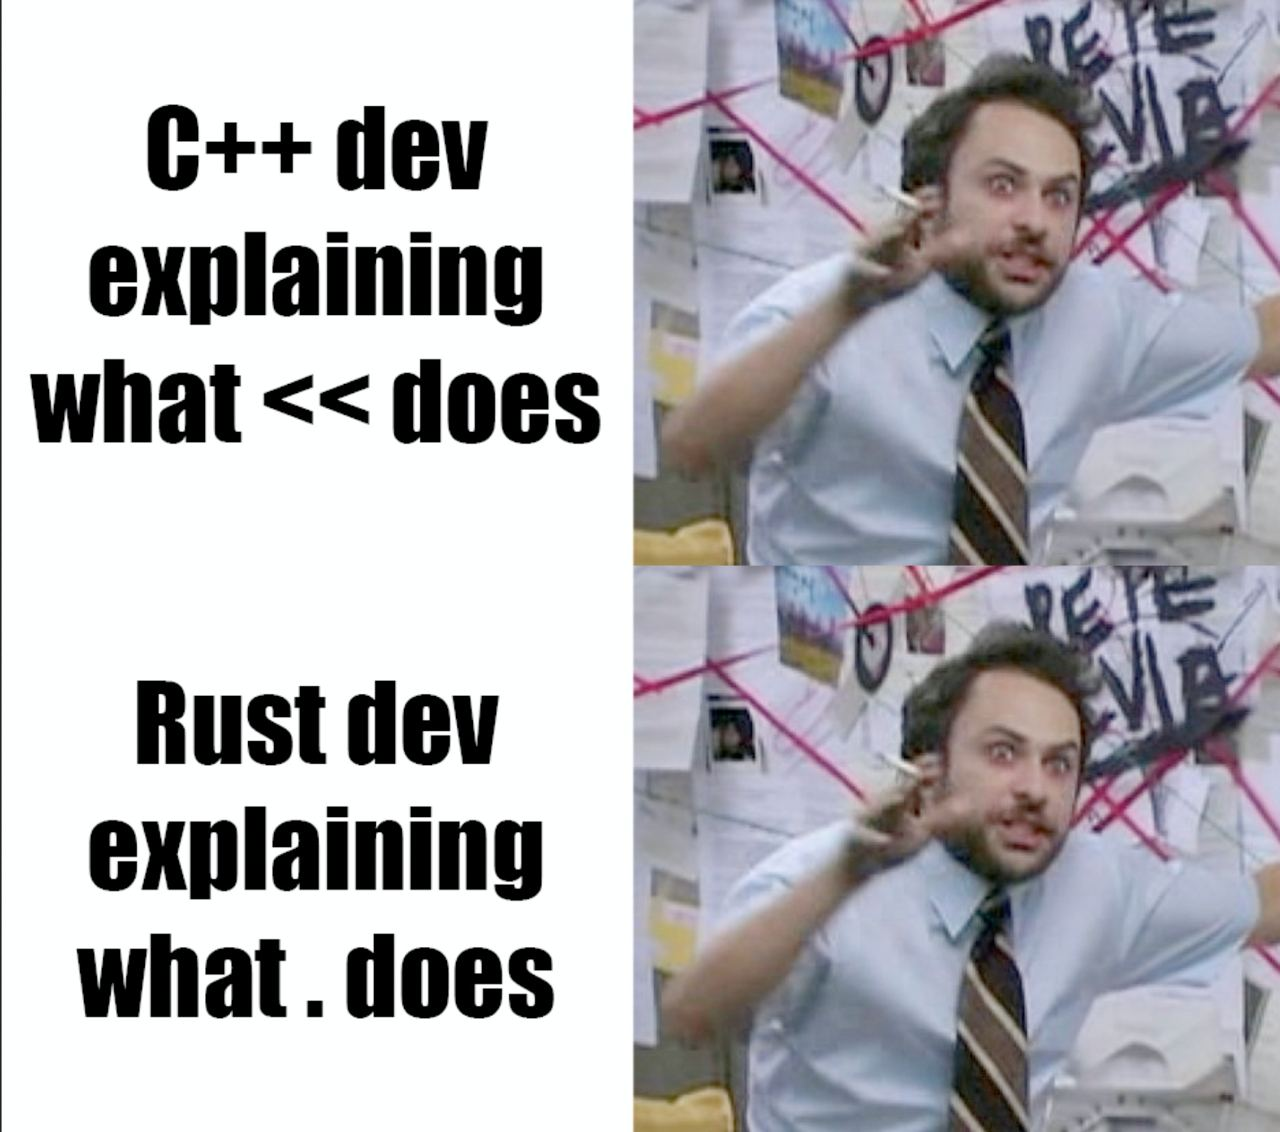
\includegraphics[height=8cm,keepaspectratio]{images/madness.jpg}
\end{frame}

% ----------------------------------------------------------------- %

\begin{frame}[fragile]
\frametitle{Dereference of \texttt{Deref}}
If \texttt{T} implements \texttt{Deref<Target = U>}, and \texttt{x} is a value of type \texttt{T}, then:

\begin{itemize}
    \item In immutable contexts, \texttt{*x} (where \texttt{T} is neither a reference nor a raw pointer) is equivalent to \texttt{*Deref::deref(\&x)}.
    \item Values of type \texttt{\&T} are coerced to values of type \texttt{\&U}.
    \item \texttt{T} implicitly implements all the (immutable) methods of the type \texttt{U}.
\end{itemize}
\end{frame}

% ----------------------------------------------------------------- %

\begin{frame}[fragile]
\frametitle{Dereference of \texttt{DerefMut}}
If \texttt{T} implements \texttt{DerefMut<Target = U>}, and \texttt{x} is a value of type \texttt{T}, then:

\begin{itemize}
    \item In mutable contexts, \texttt{*x} (where \texttt{T} is neither a reference nor a raw pointer) is equivalent to \texttt{*DerefMut::deref\_mut(\&mut x)}.
    \item Values of type \texttt{\&mut T} are coerced to values of type \texttt{\&mut U}.
    \item \texttt{T} implicitly implements all the (mutable) methods of the type \texttt{U}.
\end{itemize}
\end{frame}

% ----------------------------------------------------------------- %

\begin{frame}[fragile]
\frametitle{The dot operator}
The dot operator will perform a lot of magic to convert types. It will perform auto-referencing, auto-dereferencing, and coercion until types match.

\begin{itemize}
    \item<2-> First, the compiler checks if it can call \texttt{T::foo(value)} directly. This is called a ``by value'' method call.
    \item<3-> If it can't call this function (for example, if the function has the wrong type or a trait isn't implemented for \texttt{Self}), then the compiler tries to add in an automatic reference. This means that the compiler tries \texttt{<\&T>::foo(value)} and \texttt{<\&mut T>::foo(value)}. This is called an ``autoref'' method call.
    \item<4-> If none of these candidates worked, it dereferences \tetxtt{T} and tries again. This uses the \tetxtt{Deref} trait - if \tetxtt{T: Deref<Target = U>} then it tries again with type \tetxtt{U} instead of \tetxtt{T}. If it can't dereference \tetxtt{T}, it can also try \textbf{unsizing} \tetxtt{T}.
\end{itemize}
\end{frame}

% ----------------------------------------------------------------- %

\begin{frame}[fragile]
\frametitle{The dot operator}
Let's review the first example.

\begin{minted}{rust}
    let array: Rc<Box<[T; 3]>> = ...;
    let first_entry = array[0];
\end{minted}

\begin{enumerate}
    \item<2-> First, \texttt{array[0]} is really just syntax sugar for the \texttt{Index} trait - the compiler will convert \texttt{array[0]} into \texttt{array.index(0)}.
    \item<3-> The compiler checks if \texttt{Rc<Box<[T; 3]>>} implements \texttt{Index}, but it does not, and neither do \texttt{\&Rc<Box<[T; 3]>>} or \texttt{\&mut Rc<Box<[T; 3]>>}.
    \item<4-> The compiler dereferences the \texttt{Rc<Box<[T; 3]>>} into \texttt{Box<[T; 3]>} and tries again. \texttt{Box<[T; 3]>}, \texttt{\&Box<[T; 3]>}, and \texttt{\&mut Box<[T; 3]>} do not implement \texttt{Index}, so it dereferences again.
    \item<5-> \texttt{[T; 3]} and its autorefs also do not implement \texttt{Index}. It can't dereference \texttt{[T; 3]}, so the compiler \textbf{unsizes} it, giving \texttt{[T]}. Finally, \texttt{[T]} implements \texttt{Index}, so it can now call the actual index function.
\end{enumerate}
\end{frame}

% ----------------------------------------------------------------- %

\begin{frame}[fragile]
\frametitle{The dot operator}
Let's review the second example.

\begin{minted}{rust}
    fn do_stuff<T: Clone>(value: &T) {
        let cloned = value.clone();
    }
\end{minted}

\begin{enumerate}
    \item<2-> First, \texttt{array[0]} is really just syntax sugar for the \texttt{Index} trait - the compiler will convert \texttt{array[0]} into \texttt{array.index(0)}.
    \item<3-> The compiler checks if \texttt{Rc<Box<[T; 3]>>} implements \texttt{Index}, but it does not, and neither do \texttt{\&Rc<Box<[T; 3]>>} or \texttt{\&mut Rc<Box<[T; 3]>>}.
    \item<4-> The compiler dereferences the \texttt{Rc<Box<[T; 3]>>} into \texttt{Box<[T; 3]>} and tries again. \texttt{Box<[T; 3]>}, \texttt{\&Box<[T; 3]>}, and \texttt{\&mut Box<[T; 3]>} do not implement \texttt{Index}, so it dereferences again.
    \item<5-> \texttt{[T; 3]} and its autorefs also do not implement \texttt{Index}. It can't dereference \texttt{[T; 3]}, so the compiler \textbf{unsizes} it, giving \texttt{[T]}. Finally, \texttt{[T]} implements \texttt{Index}, so it can now call the actual index function.
\end{enumerate}
\end{frame}

% ----------------------------------------------------------------- %

\begin{frame}[fragile]
\frametitle{Comparision of traits with C++ capabilities}
\begin{itemize}
    \item<1-> Usage of traits allows us to keep the data separate from the implementation.
    \item<2-> With inheritance in C++, it is easy to introduce new types, but hard to extend with new functionality (all existing types will need to implement any new functions).
    \item<3-> Rust traits are implemented explicitly, whereas C++ concepts only require or forbid something from type.
\end{itemize}
\end{frame}

% ----------------------------------------------------------------- %

\begin{frame}[fragile]
\frametitle{Comparision of traits with C++ capabilities}
\begin{minted}[fontsize=\small]{C++}
    template<typename T>
    concept bool Stringable = requires(T a) {
        {a.stringify()} -> std::string;
    };

    class Cat {
    public:
        std::string stringify() {
            return "meow";
        }
        void pet() {}
    };

    template<Stringable T>
    void f(T a) {
        a.pet();
    }
\end{minted}
\end{frame}

% ----------------------------------------------------------------- %

\begin{frame}[fragile]
\frametitle{Comparision of traits with C++ capabilities}
This will compile just fine!

\begin{minted}[fontsize=\small]{C++}
    int main() {
        f(Cat());
        return 0;
    }
\end{minted}
\end{frame}

% ----------------------------------------------------------------- %

\begin{frame}[fragile]
\frametitle{Comparision of traits with C++ capabilities}
\begin{itemize}
    \item<1-> Usage of traits allows us to keep the data separate from the implementation.
    \item<1-> With inheritance in C++, it is easy to introduce new types, but hard to extend with new functionality (all existing types will need to implement any new functions).
    \item<1-> Rust traits are implemented explicitly, whereas C++ concepts only require or forbid something linked to type.
    \item<1-> C++ concept-constrained templates are still only type checked when concrete instantiation is attempted.
\end{itemize}
\end{frame}

% ----------------------------------------------------------------- %

\begin{frame}[c]
\centering\Huge\textbf{Interior mutability:\\\texttt{Cell} and \texttt{RefCell}}
\end{frame}

% ----------------------------------------------------------------- %

\begin{frame}[fragile]
\frametitle{Interior mutability}
Rust memory safety is based on this rule: Given an object \texttt{T}, it is only possible to have one of the following:

\begin{itemize}
    \item Having several immutable references (\texttt{\&T}) to the object (also known as aliasing).
    \item Having one mutable reference (\texttt{\&mut T}) to the object (also known as mutability).
\end{itemize}
\end{frame}

% ----------------------------------------------------------------- %

\begin{frame}[fragile]
\frametitle{Interior mutability}
But sometimes, we do want to modify the object having multiple aliases. In Rust, this is achieved using a pattern called \textit{interior mutability}.

\textbf{Important}: since Safe Rust is memory safe and does not have undefined behavior, all of these primitives must also guarantee not to break Rust's fundamental guarantees.
\end{frame}

% ----------------------------------------------------------------- %

\begin{frame}[fragile]
\frametitle{Interior mutability}
Examples:

\begin{itemize}
    \item Modifying \texttt{Rc} (main use case for this lecture).
    \item Atomics.
    \item Mutexes.
    \item RWLocks.
\end{itemize}

Basically, any mutation through \texttt{\&} is interior mutability.

In this lecture, we'll focus on \textbf{single-threaded} modification.
\end{frame}

% ----------------------------------------------------------------- %

\begin{frame}[fragile]
\frametitle{\texttt{Cell}}
Let's solve the problem by creating a safe abstraction over unsafe modification.

\begin{minted}{rust}
    pub struct Cell<T: ?Sized> {
        // ...
    }

    impl<T: Copy> Cell<T> {
        // ...
    }
\end{minted}

The \texttt{Cell} type solves this problem by \textbf{copying} the underlying value. Because of that, key functionality is \textbf{not available} when the type is not \texttt{Copy}.
\end{frame}

% ----------------------------------------------------------------- %

\begin{frame}[fragile]
\frametitle{\texttt{Cell}}
The most important functions:

\begin{minted}{rust}
    fn new(value: T) -> Cell<T>;
    fn set(&self, val: T);

    // Only when 'T: Copy'!
    fn get(&self) -> T;
\end{minted}

\texttt{set} moves the new value inside the \texttt{Cell}. \texttt{get} copies the value and gives it to the user.
\end{frame}

% ----------------------------------------------------------------- %

\begin{frame}[fragile]
\frametitle{\texttt{Cell}: Why \texttt{Copy} and not \texttt{Clone}?}
Since \texttt{Clone} allows to write any logic inside it, we can create situations when we'll cause memory unsafety and undefine behavior!

Let's use \texttt{Option} type to create a self referential \texttt{Cell} (in the example, we'll assume \texttt{Cell} is implemented for \texttt{Clone} types).\footnote{\href{https://users.rust-lang.org/t/why-does-cell-require-copy-instead-of-clone/5769/3}{Why does Cell require Copy instead of Clone?}}

\begin{minted}{rust}
    struct BadClone<'a> {
        data: i32,
        pointer: &'a Cell<Option<BadClone<'a>>>,
    }
\end{minted}
\end{frame}

% ----------------------------------------------------------------- %

\begin{frame}[fragile]
\frametitle{\texttt{Cell}: Why \texttt{Copy} and not \texttt{Clone}?}
\begin{minted}[fontsize=\small]{rust}
    impl<'a> Clone for BadClone<'a> {
        fn clone(&self) -> BadClone<'a> {
            // Grab a reference to our internals
            let data: &i32 = &self.data;
            println!("before: {}", *data);
            
            // Сlear out the cell we point to...
            self.pointer.set(None);
            
            // Print it again (should be no change!)
            println!("after: {}", *data);
            BadClone { data: self.data, pointer: self.pointer }
        }
    }
\end{minted}
\end{frame}

% ----------------------------------------------------------------- %

\begin{frame}[fragile]
\frametitle{\texttt{Cell}: Why \texttt{Copy} and not \texttt{Clone}?}
\begin{minted}{rust}
    let cell = Cell::new(None);
    cell.set(Some(BadClone {
        data: 12345678,
        pointer: &cell,
    }));
    cell.get();
\end{minted}

Possible output:

\begin{minted}{shell}
    before: 12345678
    after: 0
\end{minted}

This means the \texttt{Cell} with \texttt{Clone} is \textbf{unsound}.

More generally, this bug is called \textit{reentrancy}.
\end{frame}

% ----------------------------------------------------------------- %

\begin{frame}[fragile]
\frametitle{\texttt{RefCell}}
The \texttt{RefCell} is one more way to ensure that you correctly modify the variable.

\begin{minted}{rust}
    type BorrowFlag = isize;

    pub struct RefCell<T> 
    where
        T: ?Sized, 
    {
        borrow: Cell<BorrowFlag>,
        // ... 
    }
\end{minted}

The difference is that this type gives a mutable or immutable link and \textbf{counts these links} in runtime instead of copying the underlying type.
\end{frame}

% ----------------------------------------------------------------- %

\begin{frame}[fragile]
\frametitle{\texttt{RefCell}}
The most important functions:

\begin{minted}[fontsize=\small]{rust}
    fn new(value: T) -> RefCell<T>;
    fn get_mut(&mut self) -> &mut T;
    fn borrow(&self) -> Ref<'_, T>;
    fn borrow_mut(&self) -> RefMut<'_, T>;
    fn try_borrow(&self) -> Result<Ref<'_, T>, BorrowError>;
    fn try_borrow_mut(&self) -> Result<RefMut<'_, T>, BorrowMutError>;
\end{minted}

Structures \texttt{Ref} and \texttt{RefMut} are pinned to the \texttt{RefCell} and will change internal counter when references are dropped.

Default and \texttt{try\_} variants differs in how they notify about unsuccessful borrow: by panic or using \texttt{Result}.
\end{frame}

% ----------------------------------------------------------------- %

\begin{frame}[fragile]
\frametitle{\texttt{Cell}, \texttt{RefCell} and \texttt{Rc}}
It's quite common pattern to use \texttt{Cell} and \texttt{RefCell} together with \texttt{Rc}. \texttt{Rc}'s value is always immutable to make it safe, and if you want to modify it, you should use \texttt{Cell} or \texttt{RefCell} with runtime checks.

\begin{minted}{rust}
    pub struct List<T> {
        head: Link<T>,
        tail: Link<T>,
    }

    type Link<T> = Option<Rc<RefCell<Node<T>>>>;
\end{minted}
\end{frame}

% ----------------------------------------------------------------- %

\begin{frame}[fragile]
\frametitle{\texttt{Cell} and \texttt{RefCell} inside}
\textbf{Question}: How \texttt{Cell} and \texttt{RefCell} work?

\visible<2->{
    \textbf{Answer}: Unsafe code!
}

\begin{itemize}
    \item<2-> We'll create an unsafe structure that will give links without checking their count.
    \item<3-> And then wrap this structure into safe abstraction.
\end{itemize}

\visible<4->{
    \textbf{Note}: We are just reviewing internals of \texttt{Cell} and \texttt{RefCell}, don't use \texttt{UnsafeCell} in homeworks before we study unsafe Rust.
}
\end{frame}

% ----------------------------------------------------------------- %

\begin{frame}[fragile]
\frametitle{\texttt{Cell} and \texttt{RefCell} inside}
\begin{minted}{rust}
    pub struct UnsafeCell<T: ?Sized> {
        value: T,
    }
\end{minted}

Important functions:

\begin{minted}{rust}
    fn new(value: T) -> UnsafeCell<T>;

    // Remember: it's impossible to dereference
    // the pointer without unsafe
    fn get(&self) -> *mut T;
    fn get_mut(&mut self) -> &mut T;
\end{minted}
\end{frame}

% ----------------------------------------------------------------- %

\begin{frame}[fragile]
\frametitle{\texttt{Cell} and \texttt{RefCell} inside}
The ``true'' definitions of \texttt{Cell} and \texttt{RefCell}:

\begin{minted}{rust}
    pub struct Cell<T: ?Sized> {
        value: UnsafeCell<T>,
    }

    pub struct RefCell<T: ?Sized> {
        borrow: Cell<BorrowFlag>,
        value: UnsafeCell<T>,
    }
\end{minted}
\end{frame}

% ----------------------------------------------------------------- %

\begin{frame}[fragile]
\frametitle{\texttt{Cell} and \texttt{RefCell}: Summary}
\begin{itemize}
    \item<1-> Since it's not possible to check safe invariants on compile time when modifying from multiple places, we moved them to runtime.
    \item<2-> In the case of \texttt{Cell}, we are just copying the value, and noted impossibility of using \texttt{Clone}.
    \item<3-> In the case of \texttt{RefCell}, we are giving a reference, counting them in runtime.
    \item<4-> In C++, we must uphold ownership conditions by hand by working with references carefully.
    \item<5-> Althougth it's error prone, it's faster and requires less memory. If you need this in Rust, you should use unsafe code.
    \item<6-> Unsafe gives you the power the reponsibility of C and C++.
\end{itemize}
\end{frame}

% ----------------------------------------------------------------- %

\begin{frame}[fragile]
\frametitle{Conclusion}
\begin{itemize}
    \item We learned traits basics
    \item Studied Exotically Sized Types
    \item Reviewed standard library traits
    \item Compared of traits with C++ capabilities
    \item Understood interior mutability
\end{itemize}
\end{frame}

% ----------------------------------------------------------------- %

\end{document}
